\usetikzlibrary{patterns}

\usetikzlibrary{arrows}
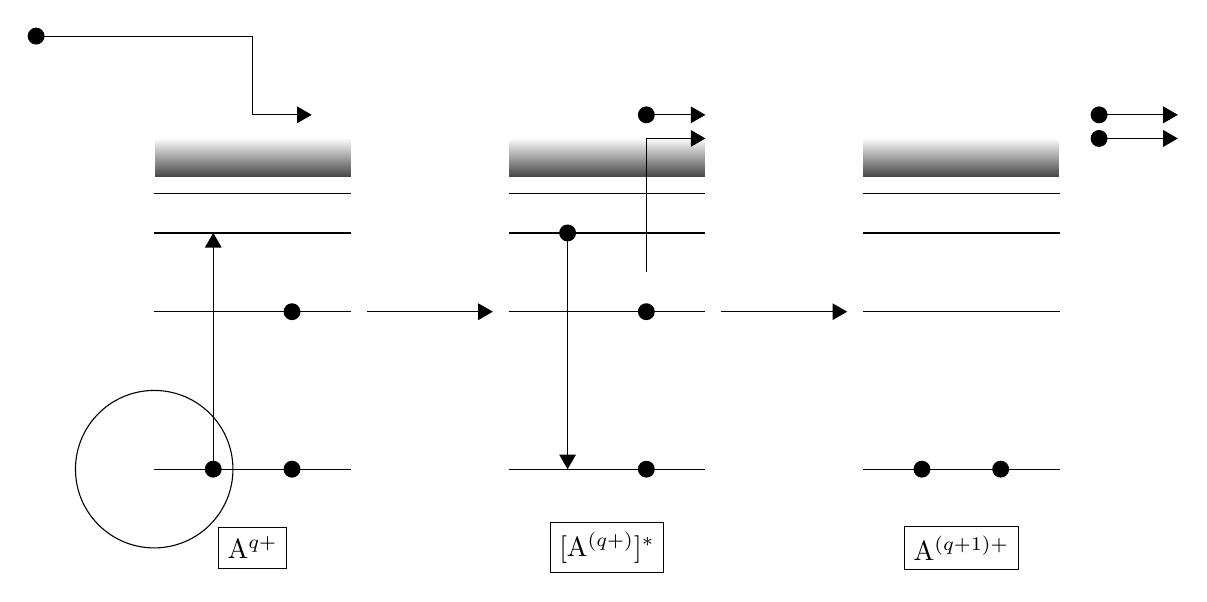
\begin{tikzpicture}
% Anker
\draw  (0,0) ellipse (1 and 1);
%

% Nr 1 Standard Darstellung ohne Elektronen
\draw (0,0) -- (2.5,0);
\draw (0,2) -- (2.5,2);
\draw (0,3) -- (2.5,3);
\draw (0,3.5) -- (2.5,3.5);
\shadedraw [draw=white,top color=lightgray!5,bottom color=darkgray] (0,3.7) rectangle (2.5,4.2);


% Nr 2 Standard Darstellung ohne Elektronen
\draw (4.5,0) -- (7,0);
\draw (4.5,2) -- (7,2);
\draw (4.5,3) -- (7,3);
\draw (4.5,3.5) -- (7,3.5);
\shadedraw [draw=white,top color=lightgray!5,bottom color=darkgray] (4.5,3.7) rectangle (7.0,4.2);


% Nr 3 Standard Darstellung ohne Elektronen
\draw (9,0) -- (11.5,0);
\draw (9,2) -- (11.5,2);
\draw (9,3) -- (11.5,3);
\draw (9,3.5) -- (11.5,3.5);
\shadedraw [draw=white,top color=lightgray!5,bottom color=darkgray] (9.0,3.7) rectangle (11.5,4.2);


% Pfeile
\draw[-triangle 60] (2.7,2) -- (4.3,2); % 1 nach 2
\draw[-triangle 60] (7.2,2) -- (8.8,2); % 2 nach 3


% Elektronen (von unten nach oben)
% Nr 1 Standard
\filldraw  (0.75,0) ellipse (0.1 and 0.1);
\filldraw  (1.75,0) ellipse (0.1 and 0.1);
\filldraw  (1.75,2.0) ellipse (0.1 and 0.1);
\filldraw  (-1.5,5.5) ellipse (0.1 and 0.1); % Kontinuum Elektron
% Elektronen (von unten nach oben)
% Nr 2 Standard
\filldraw  (6.25,0) ellipse (0.1 and 0.1);
\filldraw  (6.25,2) ellipse (0.1 and 0.1);
\filldraw  (5.25,3) ellipse (0.1 and 0.1);
\filldraw  (6.25,4.5) ellipse (0.1 and 0.1); % freie Elektronen
% Elektronen (von unten nach oben)
% Nr 3 Standard
\filldraw  (9.75,0) ellipse (0.1 and 0.1);
\filldraw  (10.75,0) ellipse (0.1 and 0.1);
\filldraw  (12,4.5) ellipse (0.1 and 0.1); % freie Elektronen
\filldraw  (12,4.2) ellipse (0.1 and 0.1); % abgelöstes Elektron 


% Elektronenweg
% Nr 1 Standard
\draw [-triangle 60](-1.5,5.5) -- (1.25,5.5) -- (1.25,4.5) -- (2.0,4.5); % Kontinuum Elektron
\draw [-triangle 60](0.75,0) -- (0.75,3);
% Elektronenweg
% Nr 2 Standard
\draw [-triangle 60](5.25,3) -- (5.25,0);
\draw [-triangle 60](6.25,2.5) -- (6.25,4.2) -- (7,4.2); % abgelöstes Elektron
\draw [-triangle 60](6.25,4.5) -- (7,4.5); % freie Elektronen
% Elektronenweg
% Nr 3 Standard
\draw [-triangle 60](12,4.5) -- (13,4.5); % abgelöstes Elektron
\draw [-triangle 60](12,4.2) -- (13,4.2); % freie Elektronen


% Beschriftung
\node[draw] at (1.25,-1) {A$^{q+}$}; % 1
\node[draw] at (5.75,-1) {[A$^{(q+)}$]$^*$}; % 2
\node[draw] at (10.25,-1) {A$^{(q+1)+}$}; % 3
\end{tikzpicture}